\documentclass[fleqn,10pt]{wlscirep}
\usepackage[utf8]{inputenc}
\usepackage[T1]{fontenc}
\usepackage{lineno}
\graphicspath{{./img/}{./pictures/}{./images/}}
\linenumbers

\usepackage[dvipsnames]{xcolor} % colors
\newcommand{\tom}[1]{{\textcolor{RedOrange}{#1}}}
\newcommand{\hh}[1]{{\textcolor{Green}{#1}}}
\usepackage{framed}

\newcommand{\ifinstruction}{1} % 1 for instruction, 0 for no instruction


% for LaTeX Error: Environment CSLReferences undefined.
%--------------------------------
% definitions for citeproc citations
\NewDocumentCommand\citeproctext{}{}
\NewDocumentCommand\citeproc{mm}{%
\begingroup\def\citeproctext{#2}\cite{#1}\endgroup}
\makeatletter
% allow citations to break across lines
\let\@cite@ofmt\@firstofone
% avoid brackets around text for \cite:
\def\@biblabel#1{}
\def\@cite#1#2{{#1\if@tempswa , #2\fi}}
\makeatother
\newlength{\cslhangindent}
\setlength{\cslhangindent}{1.5em}
\newlength{\csllabelwidth}
\setlength{\csllabelwidth}{3em}
\newenvironment{CSLReferences}[2] % #1 hanging-indent, #2 entry-spacing
{\begin{list}{}{%
	\setlength{\itemindent}{0pt}
	\setlength{\leftmargin}{0pt}
	\setlength{\parsep}{0pt}
	% turn on hanging indent if param 1 is 1
	\ifodd #1
	\setlength{\leftmargin}{\cslhangindent}
	\setlength{\itemindent}{-1\cslhangindent}
	\fi
	% set entry spacing
	\setlength{\itemsep}{#2\baselineskip}}}
{\end{list}}
\usepackage{calc}
\newcommand{\CSLBlock}[1]{\hfill\break\parbox[t]{\linewidth}{\strut\ignorespaces#1\strut}}
\newcommand{\CSLLeftMargin}[1]{\parbox[t]{\csllabelwidth}{\strut#1\strut}}
\newcommand{\CSLRightInline}[1]{\parbox[t]{\linewidth - \csllabelwidth}{\strut#1\strut}}
\newcommand{\CSLIndent}[1]{\hspace{\cslhangindent}#1}
%--------------------------------


% for gt tables
%--------------------------------
\usepackage{longtable}
%--------------------------------


%in the preamble
%--------------------------------
\usepackage[square,sort,comma,numbers]{natbib}
\bibliographystyle{jabbr}
%--------------------------------

\title{Three-dimensional data of wirecut surface scans under the
confocal microscope (110 character maximum, inc. spaces)}

\author[1,2,*]{Yuhang Lin}
\author[2,3]{Heike Hofmann}

\affil[1]{Iowa State University, Department of Statistics, Ames, }
\affil[2]{Center for Statistics and Applications in Forensic Evidence
(CSAFE), Iowa State University, Ames, }
\affil[3]{University of Nebraska-Lincoln, Department of
Statistics, Lincoln, }

      \affil[*]{corresponding author(s): Yuhang Lin (yhlin@iastate.edu)}
    
\begin{abstract}
\tom{Update later}

Wire cut data is important in forensic investigations but lacks a
systematic way of analyzing the data. We created a data set of 120 scans
of aluminum wire cut in \texttt{x3p} format, using 5 wire cutters and 3
locations along the 4 blades, with 2 replicates for each combination. A
systematic pipeline with multiple analysis plots was developed to
analyze the data and draw conclusions based on numerical measures.

\ifnum \ifinstruction=1
\fi

\textcolor{gray}{(maximum 170 words) This is a manuscript template for Data Descriptor submissions to \emph{Scientific Data} (\href{http://www.nature.com/scientificdata}{http://www.nature.com/scientificdata}). The abstract must be no longer than 170 words, and should succinctly describe the study, the assay(s) performed, the resulting data, and the reuse potential, but should not make any claims regarding new scientific findings. No references are allowed in this section.}
\end{abstract}
\begin{document}

\flushbottom
\maketitle
%  Click the title above to edit the author information and abstract

\thispagestyle{empty}

\ifnum \ifinstruction=1

\noindent \textcolor{gray}{Please note: Abbreviations should be introduced at the first mention in the main text – no abbreviations lists or tables should be included. Structure of the main text is provided below.}
\fi

\section{Background \& Summary}\label{sec-background-summary}

Wire cut data is a type of forensic tool mark data used to identify the
source of a wire cutter based on the striations left on the surface.
There have been cases where the evidence and testimony on wire cut
evidence played a crucial role in the criminal investigation and
conviction of a defendant.

However, there is a lack of a standardized method to analyze it except
for visual comparison. Although the Association of Firearm and Toolmark
Examiners (AFTE) developed the Theory of Identification (AFTE 1998)
\tom{incorrect citation format}, which outlines the process of comparing
tool marks, it is still subjective and relies on the examiner's
experience, making results hard to reproduce and validate. Several
reports, such as those from the National Research Council (NRC 2009) and
the President's Council of Advisors on Science and Technology
(President's Council of Advisors on Science and Technology 2016),
pointed out the abovementioned issues and called for more objective and
reproducible methods to analyze tool marks. Early research by (Ma et al.
2004) and (Zheng, Soons, and Thompson 2016) has focused on collecting
and distributing datasets for this purpose and providing a foundation
for future advancements in tool mark analysis. Studies such as those by
Chu et al. (2013) and Vorburger et al. (2011) have demonstrated the
efficacy of using numerical methods to improve accuracy and consistency
in tool mark analysis. Hare et al. (2017) and Ju and Hofmann (2022) have
explored methods for quantifying the similarity between representative
signals, but alignment remains a major hurdle.

In this study, we would like to follow the same path and provide a data
set of wire cut scans, and also discuss a systematic pipeline to analyze
the data and draw conclusions based on numerical measures. Here, we
provide a data set containing multiple files, as described in
Table~\ref{tbl-data-overview}.

\begin{table}

\caption{\label{tbl-data-overview}Overview of the whole data set.}

\centering{

\fontsize{12.0pt}{14.4pt}\selectfont
\begin{tabular*}{\linewidth}{@{\extracolsep{\fill}}l|ll}
\toprule
 & Description & Section \\ 
\midrule\addlinespace[2.5pt]
\multicolumn{3}{l}{Raw data} \\[2.5pt] 
\midrule\addlinespace[2.5pt]
x3p files & 120 scans of aluminum wire cut in x3p format & Cutting wires \\ 
metadata & metadata of the scans in 1 CSV & Cutting wires \\ 
\midrule\addlinespace[2.5pt]
\multicolumn{3}{l}{Manually processed derivatives} \\[2.5pt] 
\midrule\addlinespace[2.5pt]
profiles & profiles extracted from scans in 120 CSVs & Extract profiles \\ 
\midrule\addlinespace[2.5pt]
\multicolumn{3}{l}{Computational processed derivatives} \\[2.5pt] 
\midrule\addlinespace[2.5pt]
signals & signals filtered from profiles in 1 CSV & Filtered signals \\ 
aligned signals & pictures of pairwise aligned signals from same sources in PNGs & Align signals \\ 
CCF values & CCF values of all pairwise aligned signals in 1 CSV & Align signals \\ 
\bottomrule
\end{tabular*}

}

\end{table}%

\tom{breakable table, cannot cross-reference inside table}

For the reproducibility of all our data and alignment results, we
introduce in detail in Section~\ref{sec-cutting-wires}
\tom{(cross-reference not working without section number, number-sections: false not working)}
how we cut the wire and collect the 120 scans with 5 tools on 3
locations, in Section~\ref{sec-extract-profiles} how we extract profiles
from the scans, in Section~\ref{sec-filtered-signals} how we filter
signals from the profiles, in Section~\ref{sec-align-signals} how we
align signals from different scans and optimize the alignment with the
cross-correlation function (CCF) values. In
Section~\ref{sec-data-records}, we discuss where our data is held. Then,
in Section~\ref{sec-technical-validation}, a technical validation was
conducted to further compare signals from different sources also match
our assumption, together with visual aids for drawing conclusions.
Finally, in Section~\ref{sec-usage-notes}, we provide available codes
for creating the data set and conducting technical validation, as
discussed in Section~\ref{sec-methods} and
Section~\ref{sec-technical-validation}.
Section~\ref{sec-code-availability} discusses where these codes can be
found online. We hope this pipeline developed using this data set can be
further generalized and applied to real crime scenes to help
investigators draw conclusions based on real wire cut data.

\ifnum \ifinstruction=1

\textcolor{gray}{(unlimited length) An overview of the study design, the assay(s) performed, and the created data, including any background information needed to put this study in the context of previous work and the literature. The section should also briefly outline the broader goals that motivated the creation of this dataset and the potential reuse value. We also encourage authors to include a figure that provides a schematic overview of the study and assay(s) design. The Background \& Summary should not include subheadings. This section and the other main body sections of the manuscript should include citations to the literature as needed.}
\fi

\section{Methods}\label{sec-methods}

In this study, aluminum wire was used to create an optimal scenario
where the most amount of information could be transferred from the tool
to the substrate, despite the wire in some real cases being made of
lead. The physical property of aluminium wire make it an excellent
candidate for keeping marks while being relatively easy to bend and
non-toxic.

\subsection{Cutting wires}\label{sec-cutting-wires}

The aluminum wire used was 16 Gauge/1.5 mm, anodized. In order to cut
the wire, 4-inch pieces were unspooled and cut using Kaiweets wire
cutters, model KWS-105, as shown in Figure \ref{fig-cut-tent-scan}(a),
for 1 blade location, either inner, middle, or outer, which gives us 1
replicate. Each piece was then cut into half to create 2-inch pieces for
each side, AB and CD, with a sharpie line marking the cut ends, giving
us 4 samples. Here, we are showing AB sides only in Figure
\ref{fig-cut-tent-scan}(b) \tom{(remove the tent figure)}, and the CD
sides are similar from the other side of the cut, with the back of A
being C and the back of B being D. Both AB and CD sides form tent
structures on the tips of the wire, and we can separate each side of the
tent into 2 pieces along the bending position, resulting in 8 scans. We
repeated this process for all 3 locations along the blade and 5 wire
cutters, with 2 replicates for each tool-edge-location combination,
resulting in 120 scans. Each piece was labeled with the naming
conventions, T(ool) 1/2/3/4/5 (Edge) A/B/C/D W(ire) - L(ocation)
I(nner)/M(iddle)/O(uter) - R(epetition) 1/2, with T1AW-LI-R1 being the
piece cut by tool 1 on the A edge at the inner location for the first
repetition. Then, we can use the standard scanning protocols for the
confocal microscope, shown in Figure \ref{fig-cut-tent-scan}(c)
\tom{(need an extra pic of the very tip)}, to scan the wire tip
surfaces. The scanned surfaces are saved in a resolution of
\(0.645 \mu m \times 0.645 \mu m\) per square pixel in an \texttt{x3p}
file format.

\hh{XXX figure 1 - generally, zoom into these images - we do not want to have a hand in the image, nor a view of the crafting aluminum :)  - what are the exact rules on visuals in Scientific Data ? XXX}
\tom{hard to put the full requirements here, see \href{https://www.nature.com/sdata/publish/submission-guidelines\#figures}{https://www.nature.com/sdata/publish/submission-guidelines\#figures}}

\tom{put into quarto layout with (a) (b) (c) on the top left, no tent, add blade C \& D (Do later after decide on using qmd or Overleaf)}
\begin{figure}[ht]
\centering
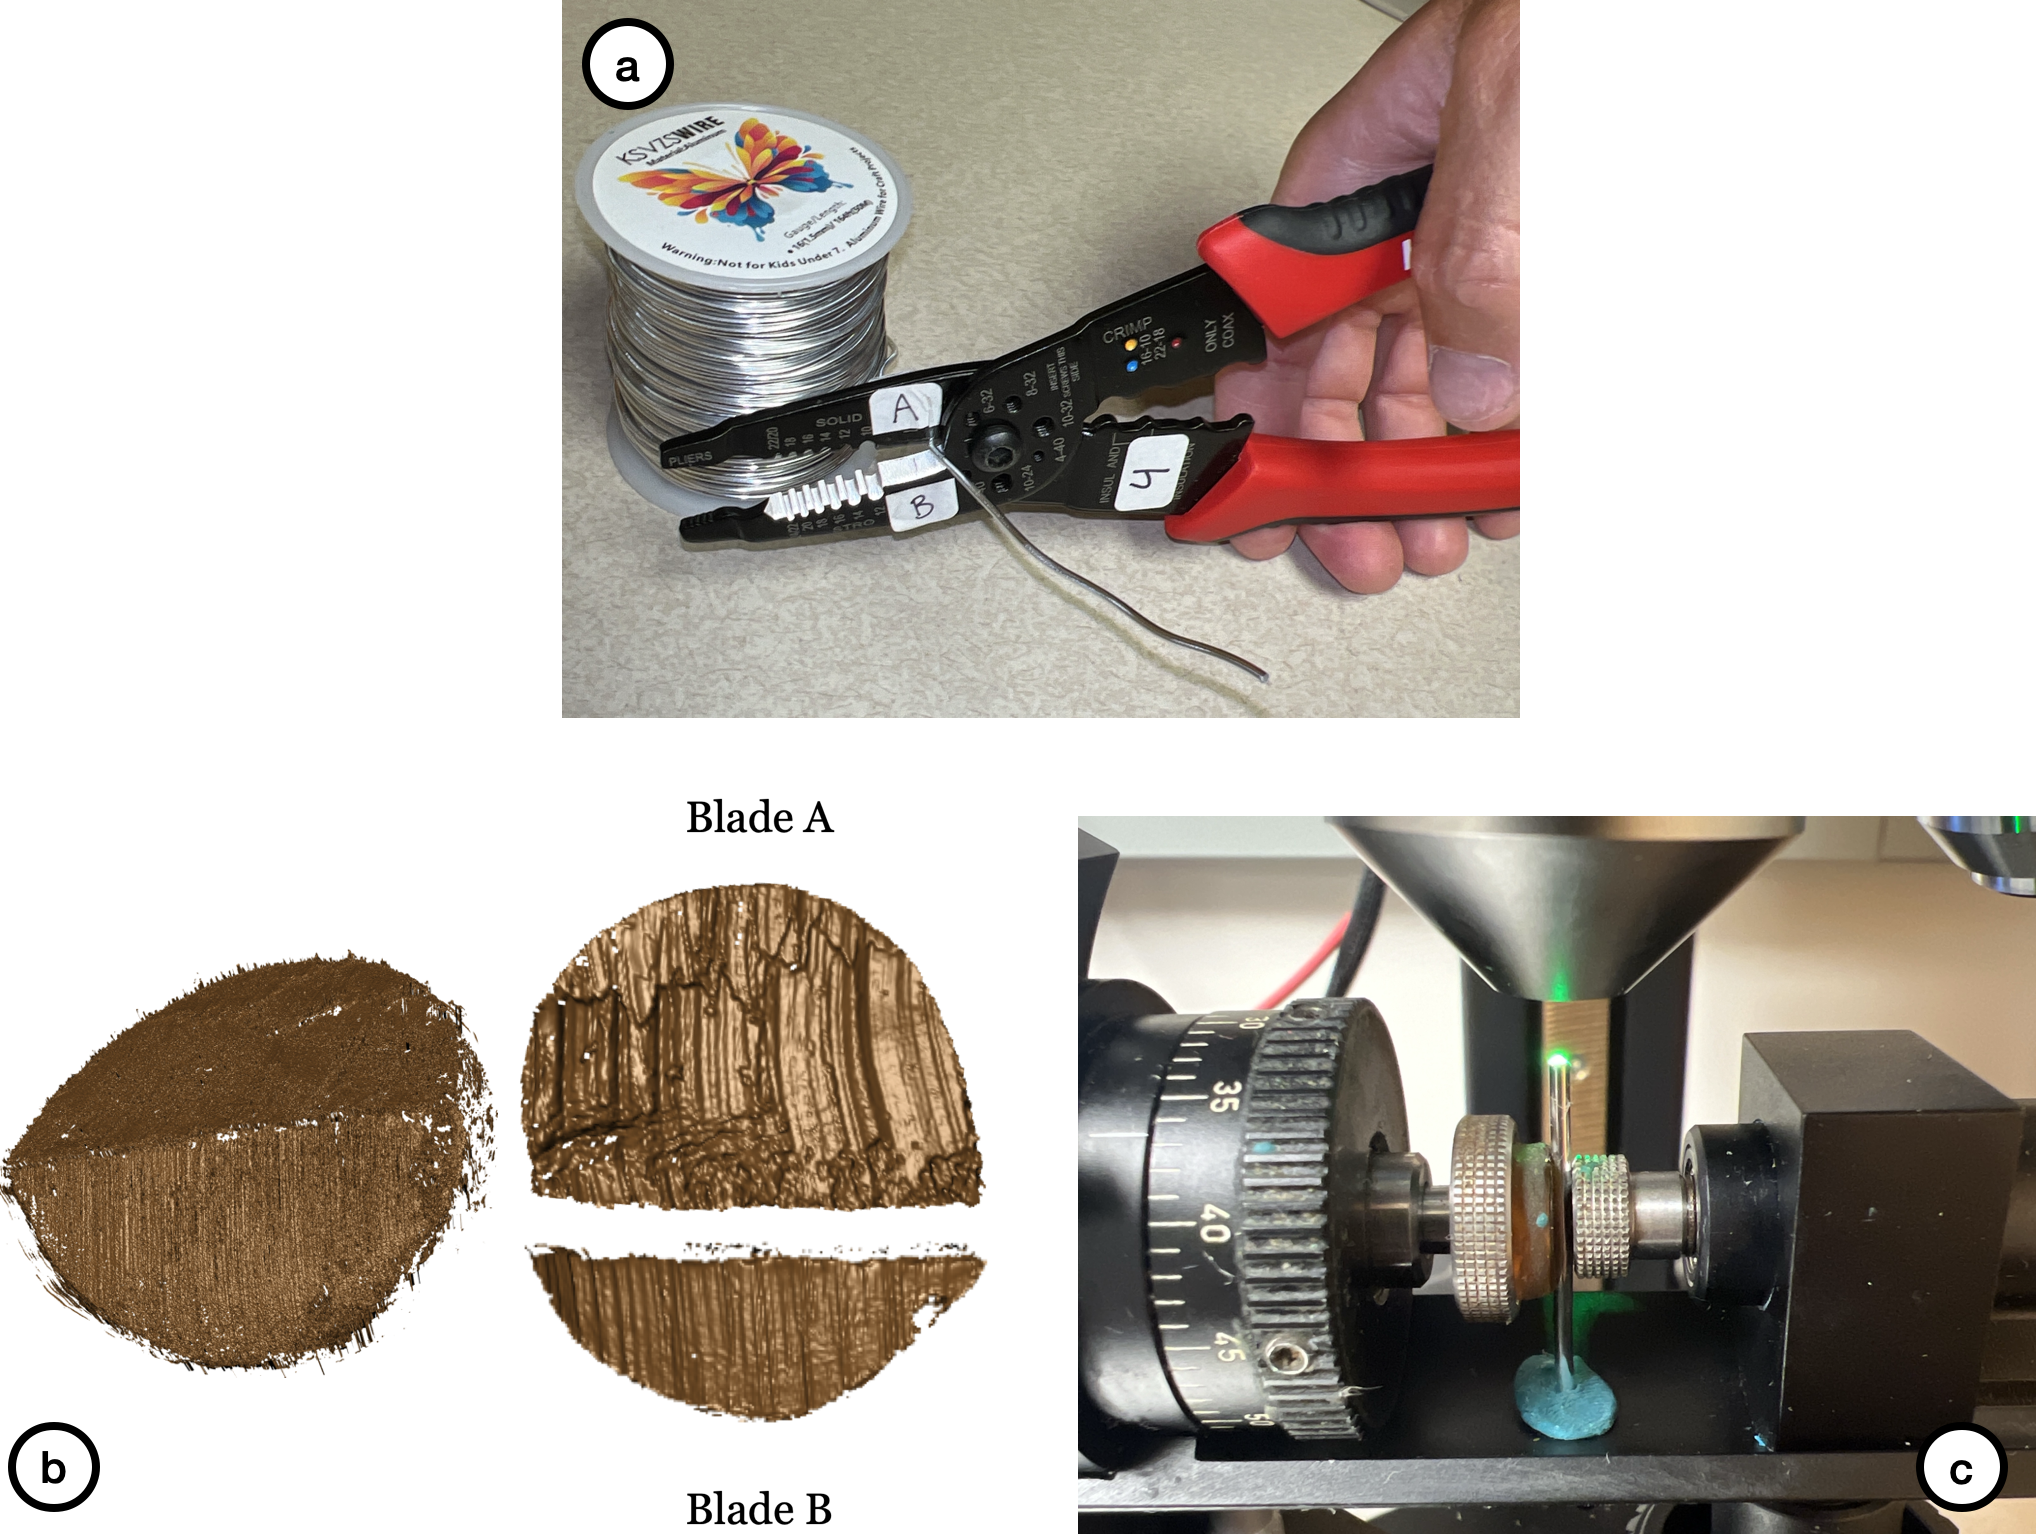
\includegraphics[width=0.9\linewidth]{cut-tent-scan.png}
\caption{(a) A Kaiweets wire cutter of model KWS-105 was used to cut the wire. (b) A tent structure created by blade AB. After separating 2 tent structures by the connecting position, we obtained 2 samples - 1 sample from blade A and B. (c) A confocal microscope was used to scan the wire surfaces.}
\label{fig-cut-tent-scan}
\end{figure}

\subsection{Extract profiles}\label{sec-extract-profiles}

Numerical comparisons between 2 replicates cannot be done directly on
the \texttt{x3p} files. We need to extract representative functions from
the scans first. A representative function with the most information is
considered as a signal for one scan, which can be used for comparison
later. To obtain this function, we first need a profile of the scan,
which is a sequence of values along a user-drawn line on the surface.
The profile should capture most features of the scan, and be orthogonal
to the striation marks of the scan, which are formed by ups and downs of
grooves. So, we draw the line across the wide region of the scan to
maximize the feature captured, as shown in dark blue in Figure
\ref{fig-T1AW-LI-R1-profiles-signals}(a). We can then investigate the
values under this profile line. The profile function is along the line
is plotted in Figure \ref{fig-T1AW-LI-R1-profiles-signals}(b).

\subsection{Filtered signals}\label{sec-filtered-signals}

With the profile extracted, we can then obtain the signal. Two Gaussian
filters are applied to these resulting profiles. In particular, we first
used a large low-pass filter with bandwidths of 400 microns to remove
large trend, as it can overwhelm the signals, and then used a small
high-pass filter of 40 microns to average across noise and remove
spikes, as shown in Figure \ref{fig-T1AW-LI-R1-profiles-signals}(c).
(Cleveland, Grosse, and Shyu 1992)
\hh{(add reference: W. S. Cleveland, E. Grosse and W. M. Shyu (1992) Local regression models. Chapter 8 of Statistical Models in S eds J.M. Chambers and T.J. Hastie, Wadsworth \& Brooks/Cole.)}.
Finally, the extreme tail values are removed.

\subsection{Align signals}\label{sec-align-signals}

Signals extracted from different scans can be put together for
comparison, and we maximize the corss-correlation function (CCF) values
between the signals to numerically find the best alignment. For example,
we compare T1AW-LI-R1 to T1AW-LI-R2, T1CW-LI-R1 to T1CW-LI-R2, and so
on. That is comparing each row in Figure \ref{fig-scans-pair}. We know
that signals from two replicates with the same tool-edge-location
combination should yield similar signals, as in the first and second
column of Figure \ref{fig-signals-pair-alignment}, which will give
alignments of massive overlapping and high CCF values close to 1. The
alignments and values we got in the rightmost column of Figure
\ref{fig-signals-pair-alignment} fulfill our expectations.

\ifnum \ifinstruction=1

\textcolor{gray}{(unlimited length) The Methods should include detailed text describing any steps or procedures used in producing the data, including full descriptions of the experimental design, data acquisition assays, and any computational processing (e.g. normalization, image feature extraction). See the detailed section in our submission guidelines for advice on writing a transparent and reproducible methods section. Related methods should be grouped under corresponding subheadings where possible, and methods should be described in enough detail to allow other researchers to interpret and repeat, if required, the full study. Specific data outputs should be explicitly referenced via data citation (see Data Records and Citing Data, below).}

\textcolor{gray}{Authors should cite previous descriptions of the methods under use, but ideally the method descriptions should be complete enough for others to understand and reproduce the methods and processing steps without referring to associated publications. There is no limit to the length of the Methods section. Subheadings should not be numbered.}

\textcolor{gray}{Authors should review the transparent methods checklist below, and ensure that their manuscript complies with any relevant points. Authors are also encouraged to search FAIRsharing.org for community reporting standards that may be relevant to their specific data-type.}

Transparent Methods Checklist

\begin{itemize}
  \item
  Materials \& reagents:
  Identify commercial suppliers of reagents, instrumentation or kits, when the source is critical to the outcome of the experiments.
  Declare any restrictions on the availability of unique materials (more information here).
  Provide catalogue or clone numbers for all antibodies (if available). For primary antibodies, provide proof of validation for the relevant species and applications.
  
  \item
  Exclusion criteria: If any data or samples were excluded, explain the exclusion criteria and state in the methods whether the criteria were established before the study was conducted.
  
  \item
  Randomization \& blinding: For any studies that involve assigning samples, animals or participants into different groups:
  State clearly whether randomization methods were used. If randomization was not employed, this should be clearly stated.
  State clearly whether blinding was employed during data collection. If blinding was not employed, this should be clearly stated.
  
  \item
  Animal \& human studies (full journal policies here):
  Experiments involving human participants must identify the committee approving the experiments, and include a statement confirming that informed consent was obtained from all participants.
  Studies employing nonhuman animals should ensure that methods descriptions comply with the ARRIVE checklist.
  
  \item
  Cell lines:
  For each eukaryotic cell line used, state the source and whether the cell line has been authenticated or otherwise tested for integrity.
  If any commonly misidentified cell lines were used (see ICLAC or NCBI Biosample), justify their use.
  Report whether the cell lines were tested for mycoplasma contamination.
  
  \item
  Chemistry \& materials science: Manuscripts describing chemical syntheses, or characterizing new chemicals or materials should refer to the guidance at Nature Chemistry.
  
\end{itemize}
\fi

\section{Data Records}\label{sec-data-records}

The complete data set is available on the ISU DataShare repository at
\href{https://iastate.figshare.com/}{https://iastate.figshare.com/},
which is public and open access for every interested researcher. The
data set consists of 120 scans in the \texttt{x3p} file format with the
naming convention as described before.
\tom{(Explain the x3p header info?)}

\ifnum \ifinstruction=1

\textcolor{gray}{(unlimited length) The Data Records section should be used to explain each data record associated with this work, including the repository where this information is stored, and to provide an overview of the data files and their formats. Each external data record should be cited numerically in the text of this section, for example \cite{Hao:gidmaps:2014}, and included in the main reference list as described below. A data citation should also be placed in the subsection of the Methods containing the data-collection or analytical procedure(s) used to derive the corresponding record. Providing a direct link to the dataset may also be helpful to readers (\hyperlink{https://doi.org/10.6084/m9.figshare.853801}{https://doi.org/10.6084/m9.figshare.853801}).}

\textcolor{gray}{Tables should be used to support the data records, and should clearly indicate the samples and subjects (study inputs), their provenance, and the experimental manipulations performed on each (please see 'Tables' below). They should also specify the data output resulting from each data-collection or analytical step, should these form part of the archived record.}
\fi

\section{Technical Validation}\label{sec-technical-validation}

\tom{a picture of alignment with ccf from different sources to show if different source, our evaluation returns small ccf, which matches what we thought.}

For the data collection process, two team members did the cutting and
labeling together, then one person did the scanning and named according
to the naming convention above. The scanning was done in a specific
order to ensure consistency across all scans. The data was saved in a
consistent format to ensure they could be easily accessed and analyzed.
A third person then checked the data to ensure that the data was
consistent in naming and accurate.

\hh{again - the website is not the right place for the validation - instead, move parts from the website here. }

\hh{For the validation of the scans and their processing we investigate the correlation scores of pair-wise aligned signals. For signals from scans of wires cut with a different tool, we would expect a low correlation score. Large scores between signals are indicative of being made by the same tool. 
Show boxplots and roc curve. }

For validation of all other tools and locations of scan replicates, see
the detailed
\href{https://heike.github.io/Wirecuts/data-descriptor/Technical_Validation.html}{report}.

\begin{figure}[ht]
\centering
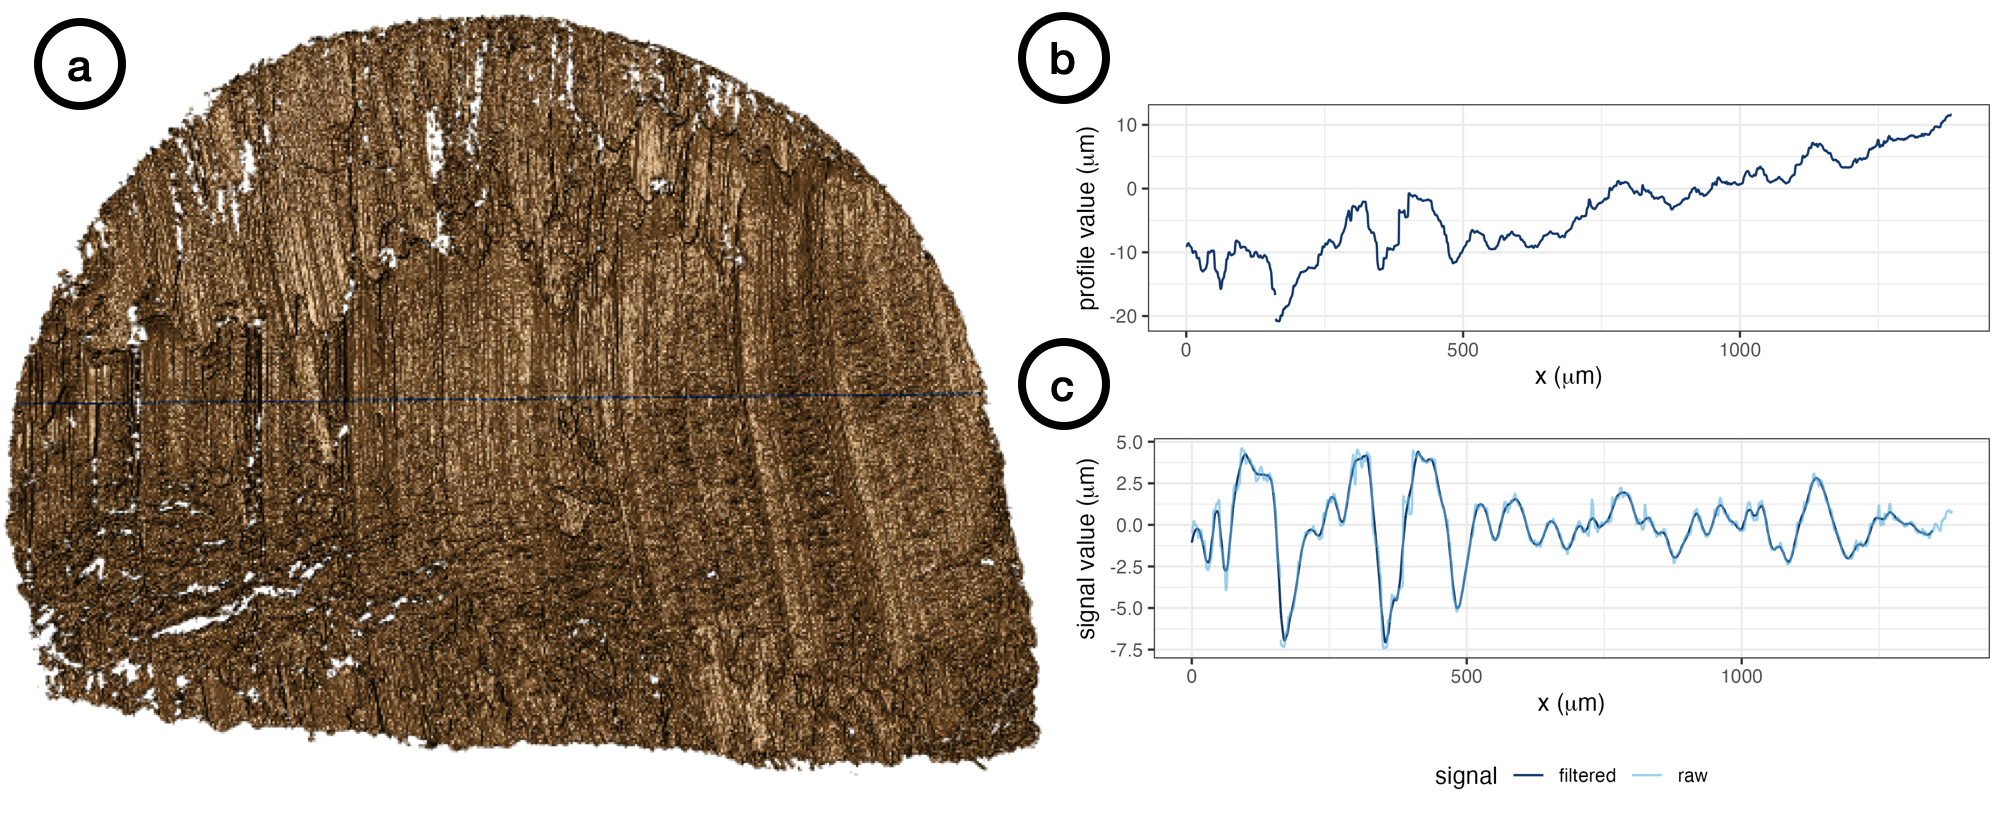
\includegraphics[width=0.9\linewidth]{T1AW-LI-R1-profiles-signals.png}
\caption{(a) A profile line in dark blue was drawn across the striations of the scan. (b) The profile function extracted along the profile line in (a). (c) The raw signal in light blue is obtained by using the low-pass filter on the profile function in (b) and the filtered signal is obtained by using the high-pass filter on the raw signal.}
\label{fig-T1AW-LI-R1-profiles-signals}
\end{figure}

\begin{figure}[ht]
\centering
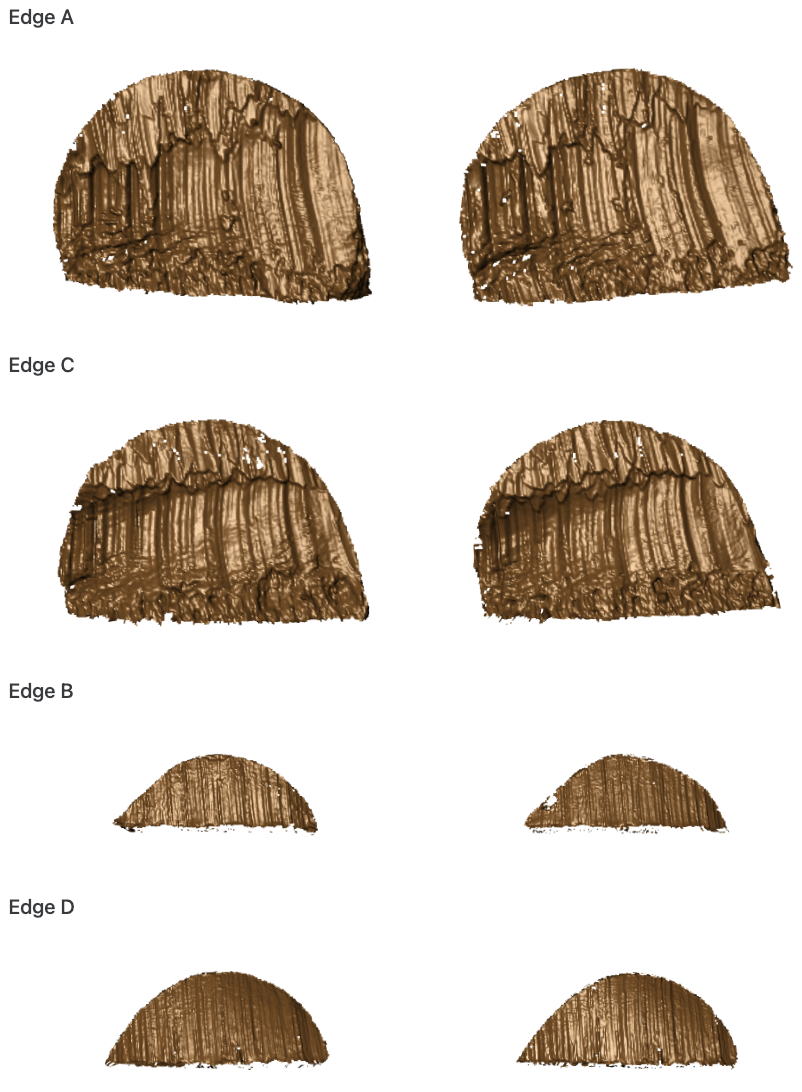
\includegraphics[width=0.8\linewidth]{scans_pair.png}
\caption{Scans from different sides of tool 1 at the inner location.}
\label{fig-scans-pair}
\end{figure}

\begin{figure}[ht]
\centering
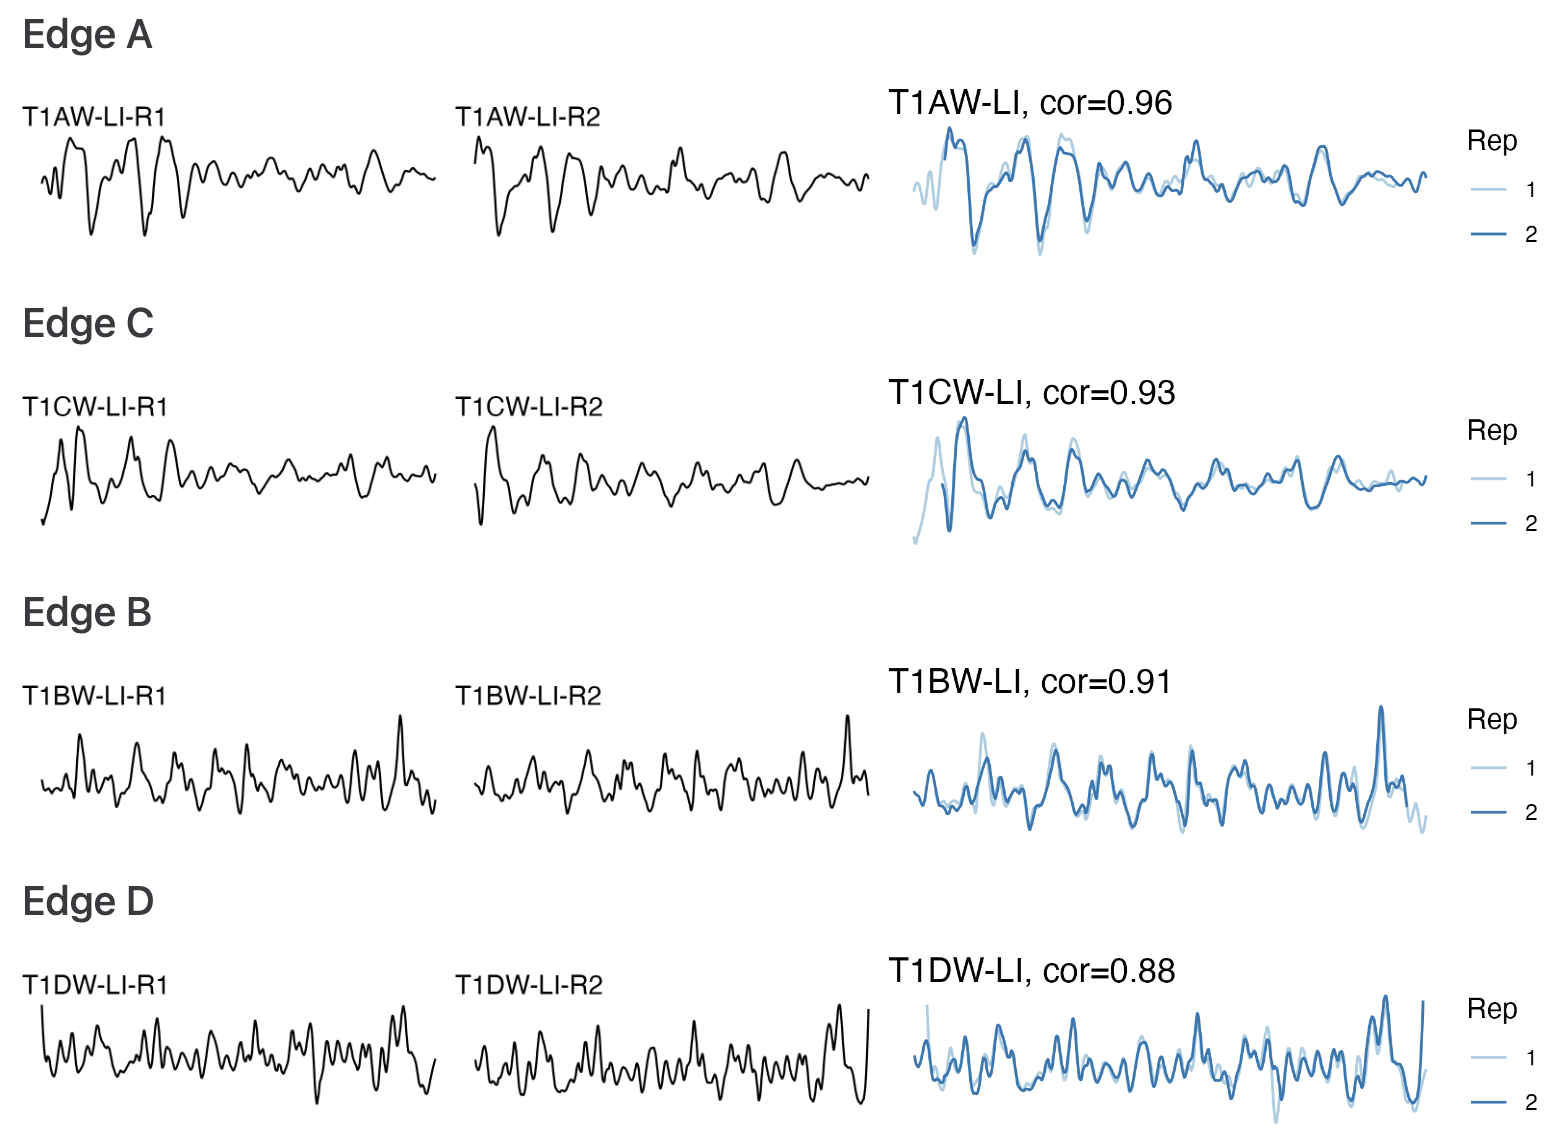
\includegraphics[width=0.8\linewidth]{signals_pair_alignment.png}
\caption{The first and second columns show the signals extracted from Figure \ref{fig-scans-pair}, and the third column shows the alignments and CCF values between pairs of signals.}
\label{fig-signals-pair-alignment}
\end{figure}

\ifnum \ifinstruction=1

\textcolor{gray}{(unlimited length) This section presents any experiments or analyses that are needed to support the technical quality of the dataset. This section may be supported by figures and tables, as needed. This is a required section; authors must present information justifying the reliability of their data.}

\begin{itemize}
  \item
  Measurement of data quality?
  
  \begin{itemize}
    \item
    Numeric measurements / tests: ?
    
    \item
    Visualizations: ?
    
    \item
    Check with existing data: ?
    
    \item
    Questionable / slur procedures:
      
      \begin{itemize}
      \item
      \href{https://www.nature.com/articles/s41597-024-03341-w?_gl=1*5ya8g2*_up*MQ..&gclid=EAIaIQobChMInOXO84DVhgMViewWBR3vWQJAEAAYASAAEgJICfD_BwE#Sec28}{AidData’s Geospatial Global Chinese Development Finance Dataset}: \textcolor{gray}{Second, all data collected is reviewed by at least two individuals. Although this is not a double-blind review procedure, the use of satellite imagery to verify project locations results in far less uncertainty when compared to previous approaches to geocoding where locations were selected entirely based on text descriptions.}
      
      \item
      \href{https://www.nature.com/articles/s41597-024-03021-9?_gl=1*1u1zppx*_up*MQ..&gclid=EAIaIQobChMInOXO84DVhgMViewWBR3vWQJAEAAYASAAEgJICfD_BwE#Sec9}{A large open access dataset of brain metastasis 3D segmentations on MRI with clinical and imaging information}: \textcolor{gray}{A medical student (D.R.) double checked and adjusted the revised NIfTI segmentation masks and manually counted the number of lesions with contrast-enhancement, necrosis, and peritumoral edema for each patient.}
      
      \item
      \href{https://www.nature.com/articles/s41597-024-03445-3?_gl=1*1ikco52*_up*MQ..&gclid=EAIaIQobChMInOXO84DVhgMViewWBR3vWQJAEAAYASAAEgJICfD_BwE#Sec11}{Time series of freshwater macroinvertebrate abundances and site characteristics of European streams and rivers}: \textcolor{gray}{Technical validation of the TREAM dataset was achieved through exclusion of time series data that did not match our inclusion criteria and data standardisation steps (outlined in Methods above). Any noted issues that did not adhere to the outlined standardisation within the datasets from the 41 independent projects included in this dataset were checked with data providers and corrected or removed when standardisation was not achievable (e.g., when collection methods changed over the course of the time series).}
      
      \item
      \href{https://www.nature.com/articles/s41597-023-02684-0?_gl=1*1t69zgo*_up*MQ..&gclid=EAIaIQobChMInOXO84DVhgMViewWBR3vWQJAEAAYASAAEgJICfD_BwE#Sec12}{3D surgical instrument collection for computer vision and extended reality}: \textcolor{gray}{The main issue...Since we store our models in a standard format (STL), they are compatible with a large variety of visualisation and processing software.}
      
      \item
      \href{https://www.nature.com/articles/s41597-024-03396-9?_gl=1*1ikco52*_up*MQ..&gclid=EAIaIQobChMInOXO84DVhgMViewWBR3vWQJAEAAYASAAEgJICfD_BwE#Sec4}{Three-dimensional reconstruction of high latitude bamboo coral via X-ray microfocus Computed Tomography
}: \textcolor{gray}{Regular quality assurance inspections are carried out on the µ-CT scanner to verify its metrological and geometrical (alignments) accuracy for conducting the scans. The geometry of source to object and source to detector distances are verified whenever there is any significant physical interaction with the source such as re-alignment, change of filament, or source anode change. This calibration process involves scanning a specially designed phantom known as an ‘hourglass’36, which consists of three pairs of high-sphericity spheres. The sphere sizes are as follows: two spheres with a diameter of 3.000 mm, two spheres with a diameter of 6.000 mm, and two spheres with a diameter of 9.525 mm, and each sphere is kept in contact with its size-counterpart. By using this phantom, it becomes possible to accurately determine a known distance, specifically the centre-to-centre distance of the spheres, in a threshold-independent manner. If the measured distance deviates beyond the acceptable limits of metrological accuracy, the system’s calibration parameters are adjusted to ensure agreement between the measured distance and the actual distance.}
      
      \end{itemize}
      
    \end{itemize}
  
\end{itemize}
\fi

\section{Usage Notes}\label{sec-usage-notes}

\hh{The \texttt{R} package \texttt{x3ptools} (available from \texttt{CRAN}) supports working with files in  x3p format. }

\hh{Sample scripts in R for processing scans from x3p format to their signal are available from ... github. }

Further analysis can be conducted with the \texttt{GitHub} \texttt{R}
package \texttt{wire} and the \texttt{GitHub} \texttt{R} shiny app
\texttt{wireShiny} \tom{(citation?)}. We already conduct
between-replicate comparisons in the technical validation section, and
we can also conduct across-replicate comparisons to establish error
rates threshold and produce other analysis plots.

Suppose we put the CCF values in a tilemap with different tool, location
and edge combinations. In that case, we expect only the diagonal to have
high CCF values, close to 1 and marked as orange in the tilemap, as the
diagonal represents the same source, and the rest of the matrix to have
low CCF values, close to 0 and marked as gray. In Figure
\ref{fig-ccf-tilemap}, the behavior is consistent with our expectation
overall, except for some rare cases with tool 5 edge D, which is caused
by \tom{?????}. We also put the resulting CCFs in the boxplot, as in
Figure \ref{fig-ccf-boxplot}. We can see that the CCF values for the
same sources are close to 1, while the CCF values for different sources
are much lower than expected. This difference can be used to establish a
threshold for CCF and help us draw conclusions about the similarity
between wire cut scans numerically, which can be used in real crime
scenes. The density plot in Figure \ref{fig-ccf-density} shows the
distribution of the CCF values with the same sources and different
sources. The overlapping points between the tails of these two
distributions can be a rough threshold. Furthermore, the receiver
operating characteristic (ROC) curve in Figure \ref{fig-ccf-ROC} shows
the sensitivity / true positive rate against the false positive rate
(FPR) (1 - specificity). The curve is very close to the upper left
corner, which is excellent for classification and drawing conclusion. It
gives us a true threshold of 0.589 to control the FPR to be less than
0.05 with false negative rate (FNR) to be 0,
\tom{(false positive rate (FPR) / false discovery rate (FDR) -> define the H0 or call it false identification rate (FIR)???)},
and 0.658 to control the FPR to be less than 0.01, with FNR to be 0.02.

\begin{figure}[ht]
\centering
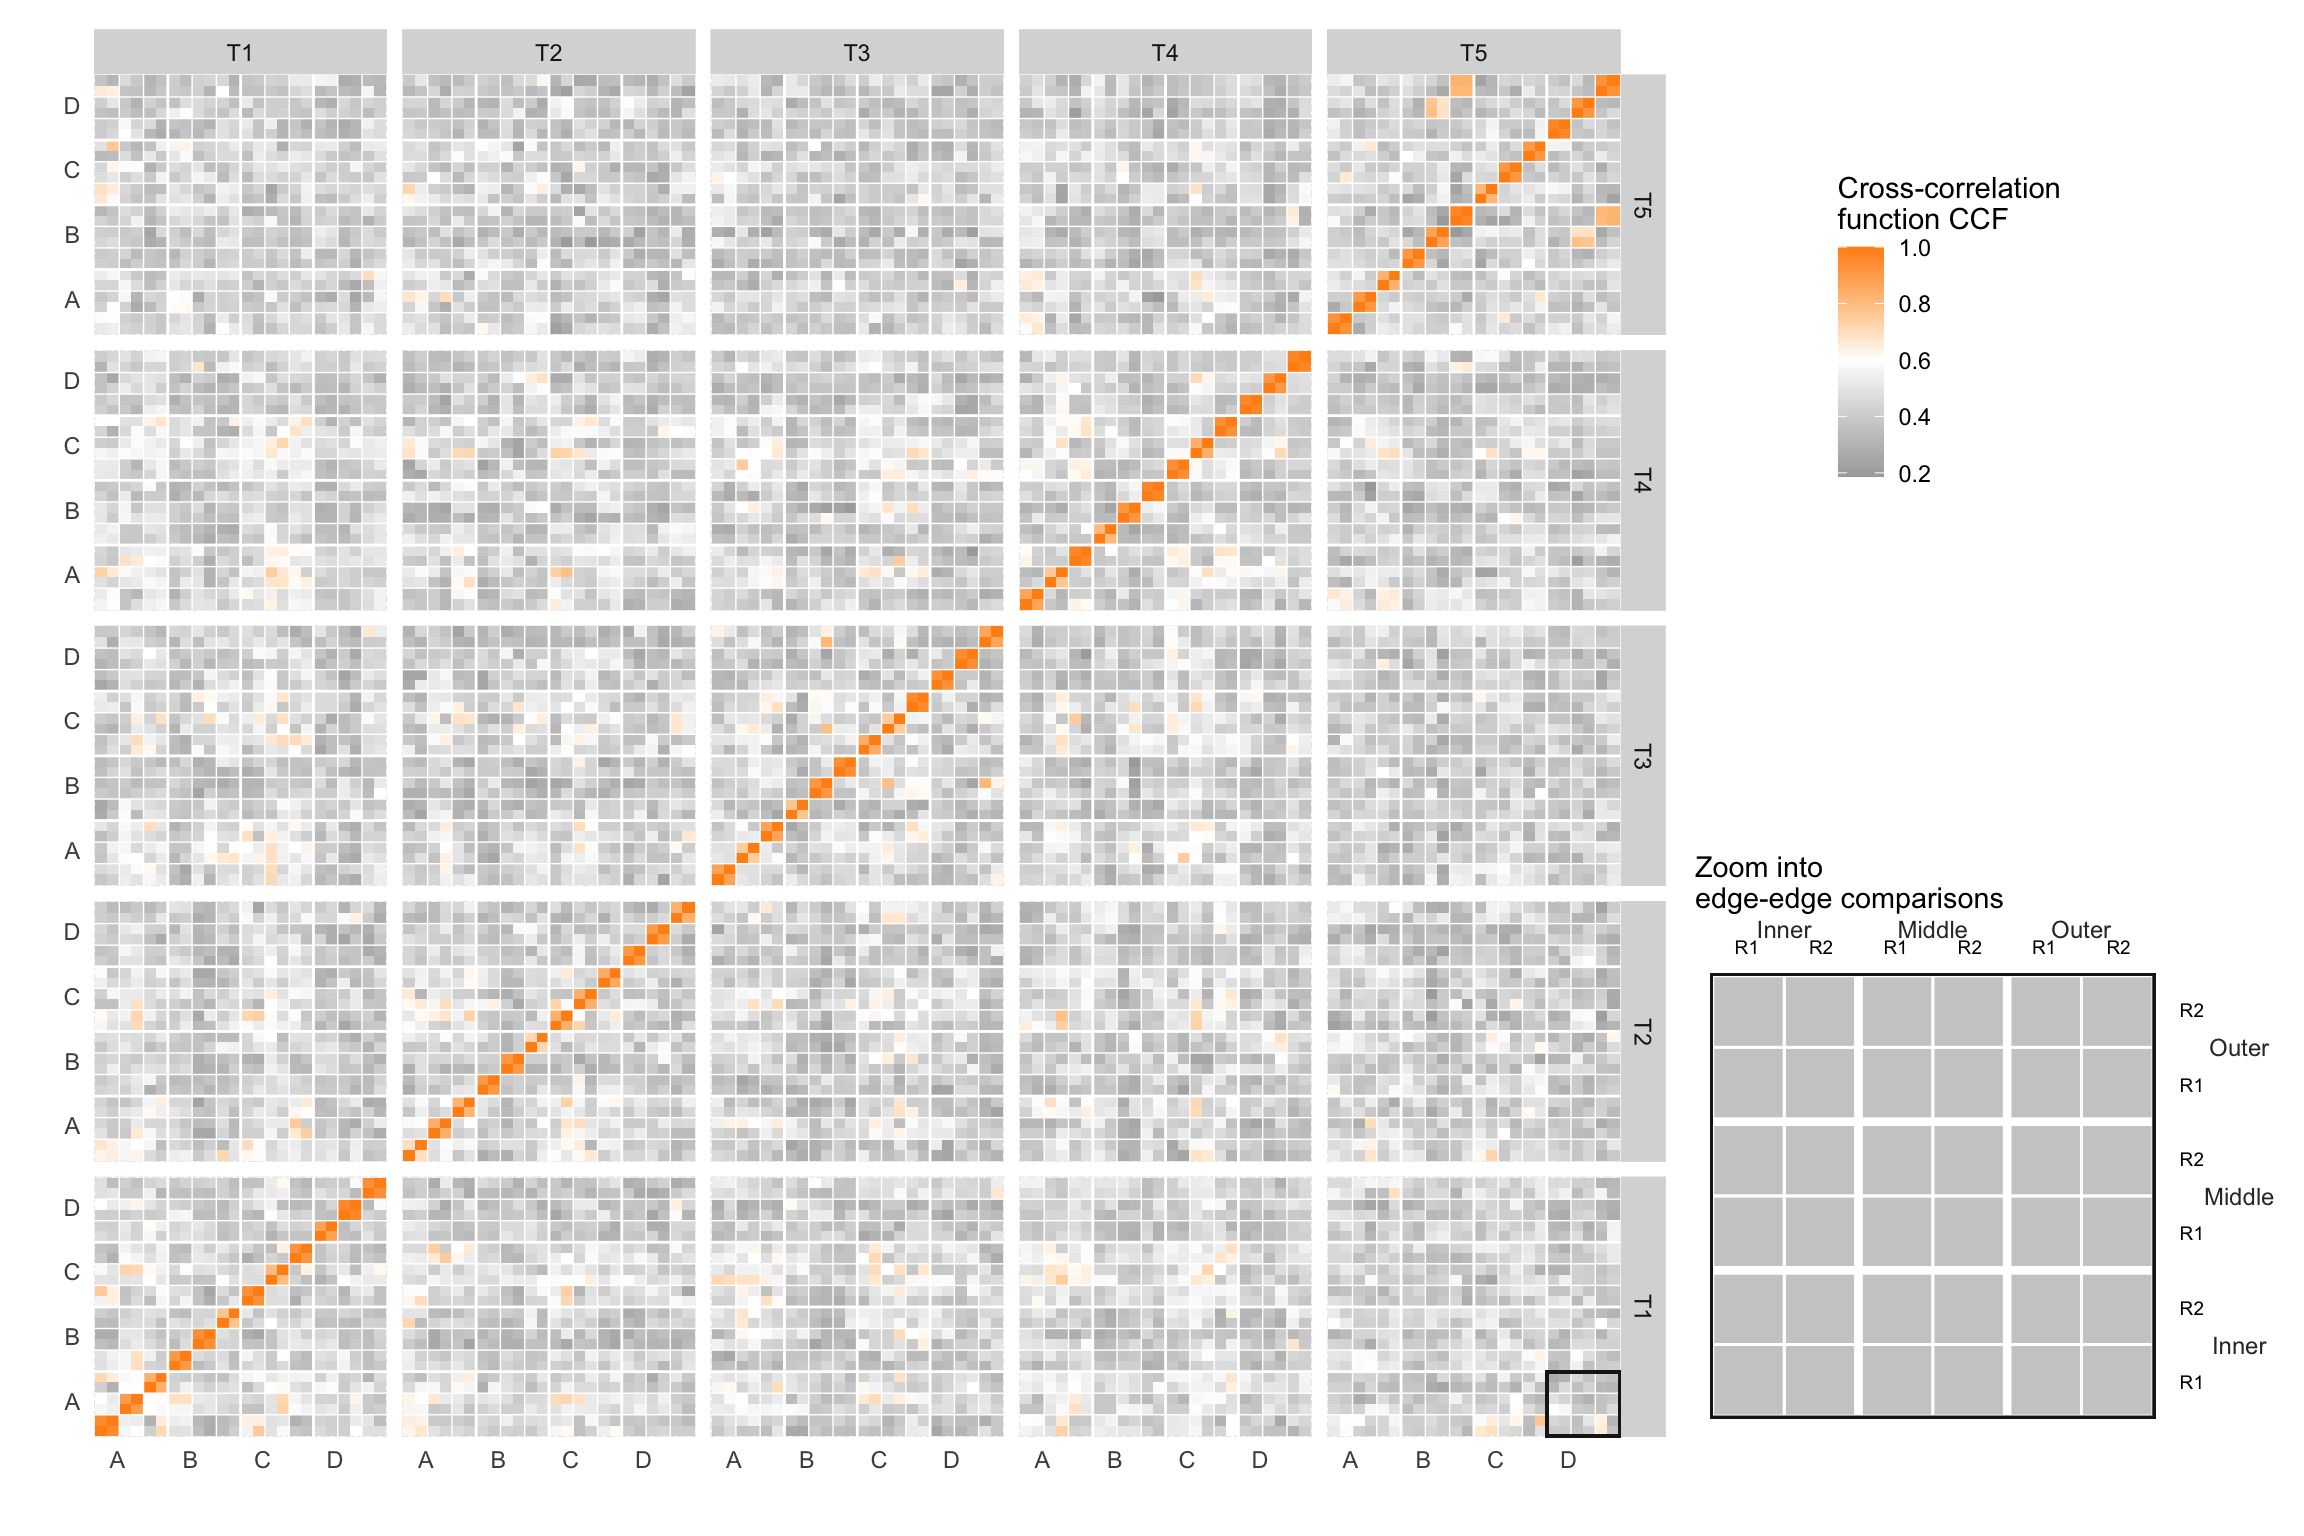
\includegraphics[width=0.8\linewidth]{ccf_tilemap.png}
\caption{The tilemap shows signals from the same source have CCFs close to 1.}
\label{fig-ccf-tilemap}
\end{figure}

\begin{figure}[ht]
\centering
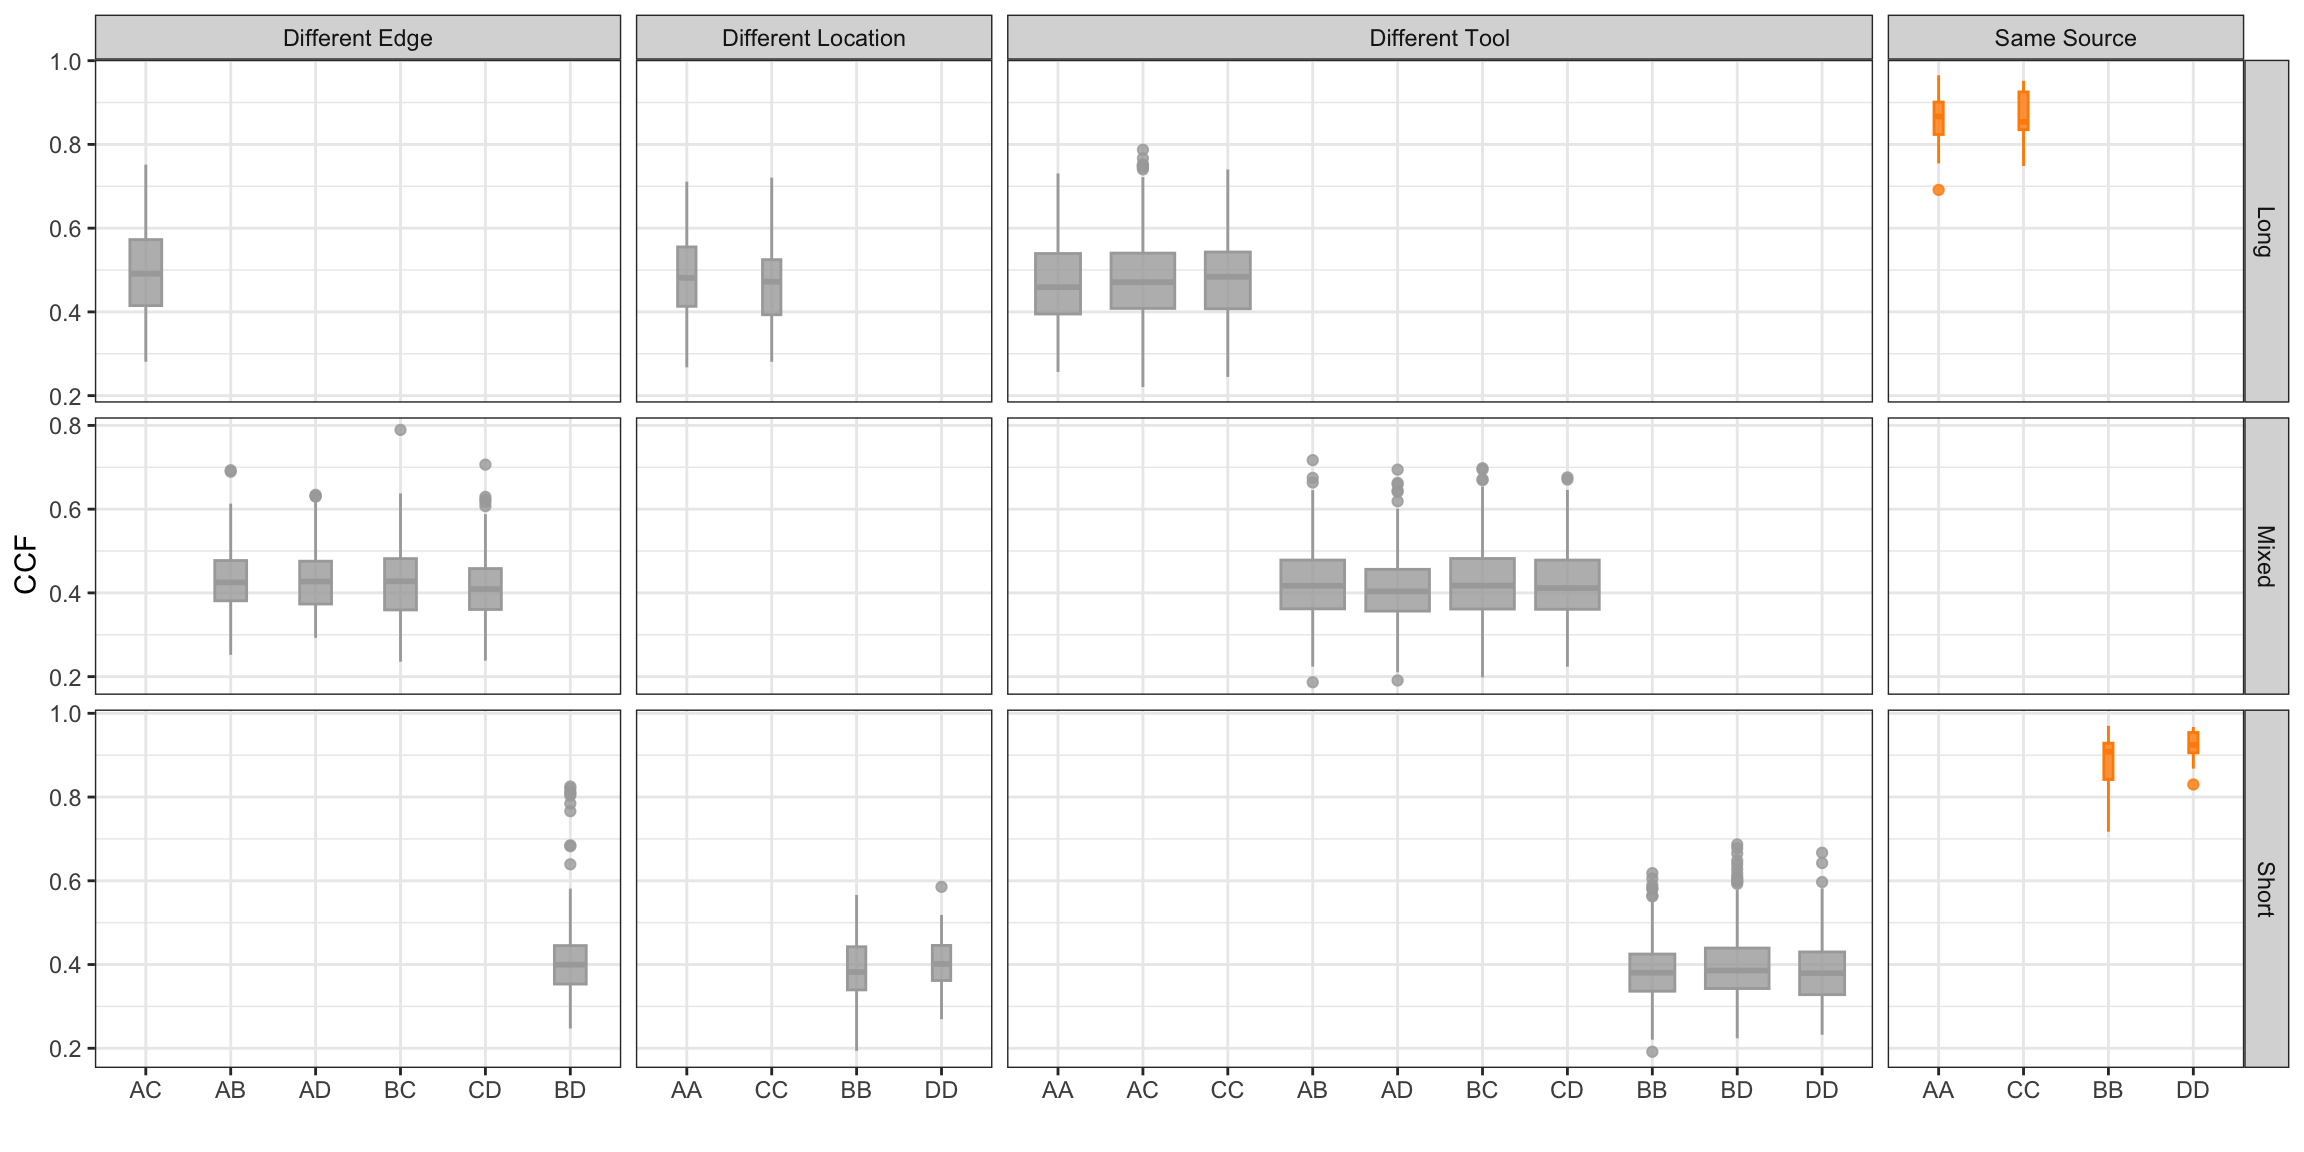
\includegraphics[width=0.8\linewidth]{ccf_boxplot.png}
\caption{The boxplot shows that signals from the same sources have higher CCfs than those from different sources.}
\label{fig-ccf-boxplot}
\end{figure}

\begin{figure}[ht]
\centering
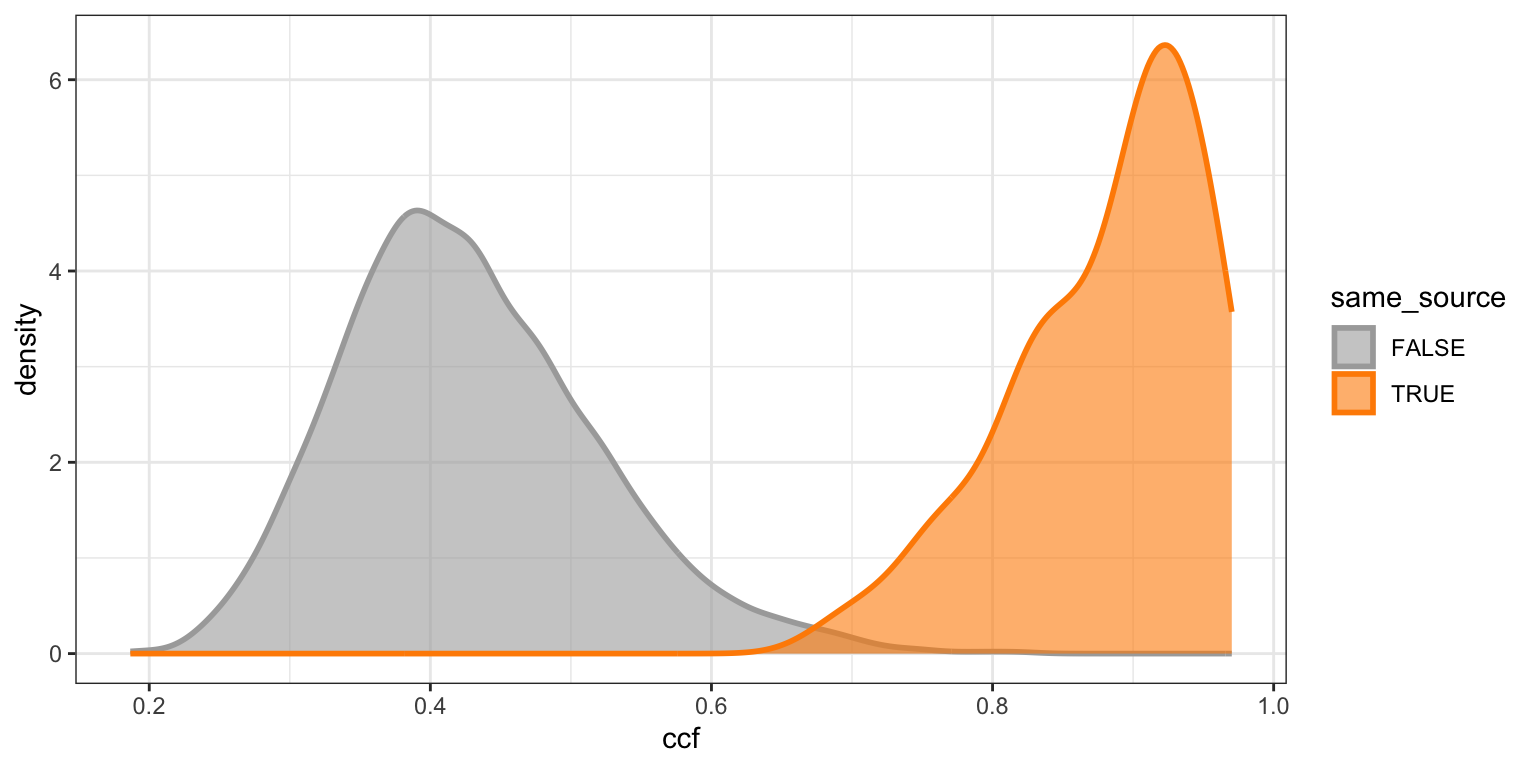
\includegraphics[width=0.8\linewidth]{ccf_density.png}
\caption{The density plot shows tails of distributions overlap, which can be used as a rough threshold for drawing conclusions.}
\label{fig-ccf-density}
\end{figure}

\begin{figure}[ht]
\centering
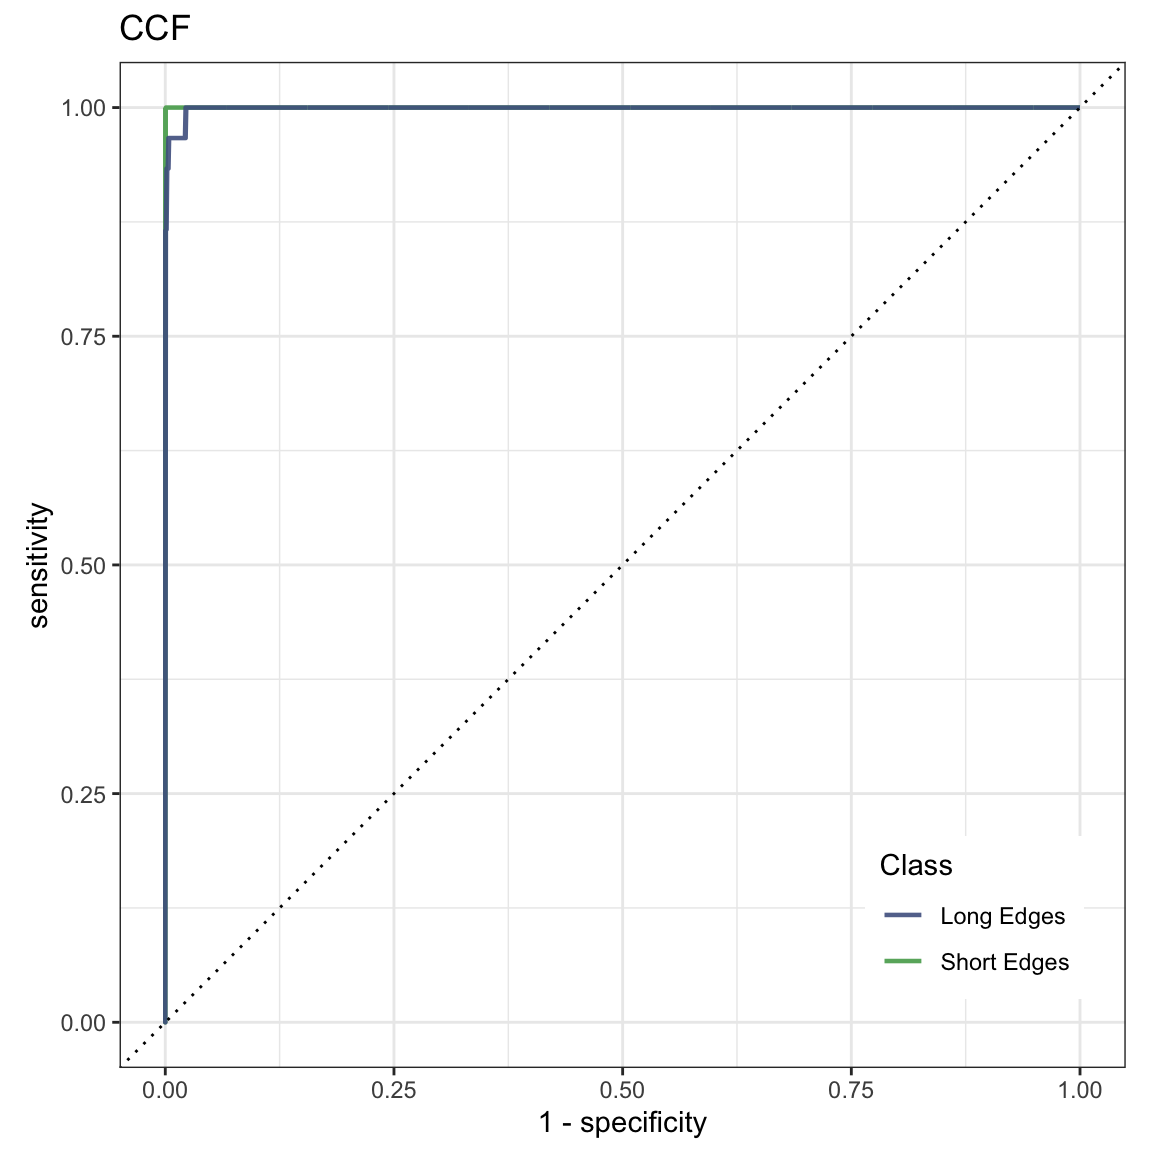
\includegraphics[width=0.5\linewidth]{ccf_ROC.png}
\caption{The ROC curve is bending very close to the upper left corner, which means excellent in classification and drawing conclusions.}
\label{fig-ccf-ROC}
\end{figure}

\ifnum \ifinstruction=1

\textcolor{gray}{(unlimited length) The Usage Notes should contain brief instructions to assist other researchers with reuse of the data. This may include discussion of software packages that are suitable for analysing the assay data files, suggested downstream processing steps (e.g. normalization, etc.), or tips for integrating or comparing the data records with other datasets. Authors are encouraged to provide code, programs or data-processing workflows if they may help others understand or use the data. Please see our code availability policy for advice on supplying custom code alongside Data Descriptor manuscripts.}

\textcolor{gray}{For studies involving privacy or safety controls on public access to the data, this section should describe in detail these controls, including how authors can apply to access the data, what criteria will be used to determine who may access the data, and any limitations on data use.}
\fi

\section{Code availability}\label{sec-code-availability}

\tom{table of code-manual?}

\hh{no, we can't use the website as a place for more detailed procedures. This paper is the detailed procedure.}\tom{no more README, scanning procedures in another HTML}

We put together the cutting and the standard scanning procedures
mentioned in Section \ref{sec-cutting-wires} \tom{cross-ref not working}
with more pictures for each step into a
\href{https://github.com/heike/Wirecuts/blob/main/README.md}{README of the GitHub repository \texttt{heike/Wirecuts}}
\tom{(High-res pics needed in the README)}.

The data set can be easily accessed with the \texttt{CRAN} \texttt{R}
package \texttt{x3ptools}. Further analysis can be conducted with the
\texttt{GitHub} \texttt{R} package \texttt{wire} and the \texttt{GitHub}
\texttt{R} shiny app \texttt{wireShiny} \tom{(citation)}
\tom{(again????)}.

\ifnum \ifinstruction=1

\textcolor{gray}{For all studies using custom code in the generation or processing of datasets, a statement must be included under the heading "Code availability", indicating whether and how the code can be accessed, including any restrictions to access. This section should also include information on the versions of any software used, if relevant, and any specific variables or parameters used to generate, test, or process the current dataset.}
\fi

\section{End of Body}\label{end-of-body}

\hh{(Note that the bibliography style and the name of the bib-file are hard coded in the template file right now.)}

\phantomsection\label{refs}
\begin{CSLReferences}{1}{0}
\bibitem[\citeproctext]{ref-afte}
AFTE. 1998. {``The Association of Firearm and Tool Mark Examiners:
{Theory} of Identification as It Relates to Toolmarks.''} \emph{AFTE
Journal} 30 (1): 86--88.

\bibitem[\citeproctext]{ref-chuAutomaticIdentificationBullet2013}
Chu, Wei, Robert M. Thompson, John Song, and Theodore V. Vorburger.
2013. {``Automatic Identification of Bullet Signatures Based on
Consecutive Matching Striae ({CMS}) Criteria.''} \emph{Forensic Science
International} 231 (1-3): 137--41. \url{https://doi.org/gn65cz}.

\bibitem[\citeproctext]{ref-clevelandLocalRegressionModels1992}
Cleveland, William S., Eric Grosse, and William M. Shyu. 1992. {``Local
{Regression Models}.''} In \emph{Statistical {Models} in {S}}.
Routledge.

\bibitem[\citeproctext]{ref-hareAutomaticMatchingBullet2017}
Hare, Eric, Heike Hofmann, Alicia Carriquiry, et al. 2017. {``Automatic
Matching of Bullet Land Impressions.''} \emph{The Annals of Applied
Statistics} 11 (4): 2332--56. \url{https://doi.org/10.1214/17-AOAS1080}.

\bibitem[\citeproctext]{ref-juJournalOpenSourceImplementation2022}
Ju, Wangqian, and Heike Hofmann. 2022. {``The {R Journal}: {An
Open-Source Implementation} of the {CMPS Algorithm} for {Assessing
Similarity} of {Bullets}.''} \emph{The R Journal} 14 (2): 267--85.
\url{https://doi.org/10.32614/RJ-2022-035}.

\bibitem[\citeproctext]{ref-maNISTBulletSignature2004}
Ma, Li, John Song, Eric Whitenton, Alan Zheng, Theodore Vorburger, and
Jack Zhou. 2004. {``{NIST Bullet Signature Measurement System} for {RM}
({Reference Material}) 8240 {Standard Bullets}.''} \emph{Journal of
Forensic Sciences} 49 (4): 1--11. \url{https://doi.org/cdsbv8}.

\bibitem[\citeproctext]{ref-nas2009}
NRC. 2009. \emph{National Research Council: {Strengthening} Forensic
Science in the United States: {A} Path Forward}. National Academies
Press.

\bibitem[\citeproctext]{ref-pcast}
President's Council of Advisors on Science and Technology. 2016.
\emph{President's Council of Advisors on Science and Technology:
{Forensic} Science in Criminal Courts: {Ensuring} Scientific Validity of
Feature-Comparison Methods}. Washington, D.C.: Executive Office of the
President of the United States, President's Council.
\url{https://obamawhitehouse.archives.gov/sites/default/files/microsites/ostp/PCAST/pcast_forensic_science_report_final.pdf}.

\bibitem[\citeproctext]{ref-vorburgerApplicationsCrosscorrelationFunctions2011}
Vorburger, T. V., J.-F. Song, W. Chu, L. Ma, S. H. Bui, A. Zheng, and T.
B. Renegar. 2011. {``Applications of Cross-Correlation Functions.''}
\emph{Wear} 271 (3-4): 529--33. \url{https://doi.org/dt4kzk}.

\bibitem[\citeproctext]{ref-zhengNISTBallisticsToolmark2016}
Zheng, Xiaoyu A., Johannes A. Soons, and Robert M. Thompson. 2016.
{``{NIST Ballistics Toolmark Research Database} {\textbar} {NIST}.''}
\url{https://www.nist.gov/publications/nist-ballistics-toolmark-research-database}.

\end{CSLReferences}

\bibliography{references}

\noindent LaTeX formats citations and references automatically using the bibliography records in your .bib file, which you can edit via the project menu. Use the cite command for an inline citation, e.g. \cite{Kaufman2020, Figueredo:2009dg, Babichev2002, behringer2014manipulating}. For data citations of datasets uploaded to e.g. \emph{figshare}, please use the \verb|howpublished| option in the bib entry to specify the platform and the link, as in the \verb|Hao:gidmaps:2014| example in the sample bibliography file. For journal articles, DOIs should be included for works in press that do not yet have volume or page numbers. For other journal articles, DOIs should be included uniformly for all articles or not at all. We recommend that you encode all DOIs in your bibtex database as full URLs, e.g. https://doi.org/10.1007/s12110-009-9068-2.

\section*{Acknowledgements} 
\ifnum \ifinstruction=1

Acknowledgements should be brief, and should not include thanks to
anonymous referees and editors, or effusive comments. Grant or
contribution numbers may be acknowledged. \fi

\section*{Author contributions statement}

\ifnum \ifinstruction=1
\fi

Y.L. did all of the work, H.H. made him do the work. But seriously, this
paper is the one where we need to cite everybody: Eden Amin, Curtis
Mosher, Jeff Salyards. Alicia?
Must include all authors, identified by initials, for example:
A.A. conceived the experiment(s), A.A. and B.A. conducted the experiment(s), C.A. and D.A. analysed the results. All authors reviewed the manuscript. 

\section*{Competing interests} (mandatory statement)

\ifnum \ifinstruction=1

H.H. is a technical advisor to AFTE (Association of Firearms and
Toolmarks Examiners), fellow of the ASA (American Statistical
Association), and committee member of the ASA Forensic Science
Committee. H.H. has testified as court witness on behalf of judge April
Neubauer, NY State Supreme Court Criminal Term in New York City. \fi The
corresponding author is responsible for providing a
\href{https://www.nature.com/sdata/policies/editorial-and-publishing-policies#competing}{competing interests statement}
on behalf of all authors of the paper. This statement must be included
in the submitted article file.

% XXX Delete the section below later
\ifnum \ifinstruction=1
\section*{Figures \& Tables}


Figures, tables, and their legends, should be included at the end of the document. Figures and tables can be referenced in \LaTeX{} using the ref command, e.g. Figure \ref{fig:stream} and Table \ref{tab:example}. 

Authors are encouraged to provide one or more tables that provide basic information on the main ‘inputs’ to the study (e.g. samples, participants, or information sources) and the main data outputs of the study. Tables in the manuscript should generally not be used to present primary data (i.e. measurements). Tables containing primary data should be submitted to an appropriate data repository.

Tables may be provided within the \LaTeX{} document or as separate files (tab-delimited text or Excel files). Legends, where needed, should be included here. Generally, a Data Descriptor should have fewer than ten Tables, but more may be allowed when needed. Tables may be of any size, but only Tables which fit onto a single printed page will be included in the PDF version of the article (up to a maximum of three). 

Due to typesetting constraints, tables that do not fit onto a single A4 page cannot be included in the PDF version of the article and will be made available in the online version only. Any such tables must be labelled in the text as ‘Online-only’ tables and numbered separately from the main table list e.g. ‘Table 1, Table 2, Online-only Table 1’ etc.

\begin{figure}[ht]
\centering
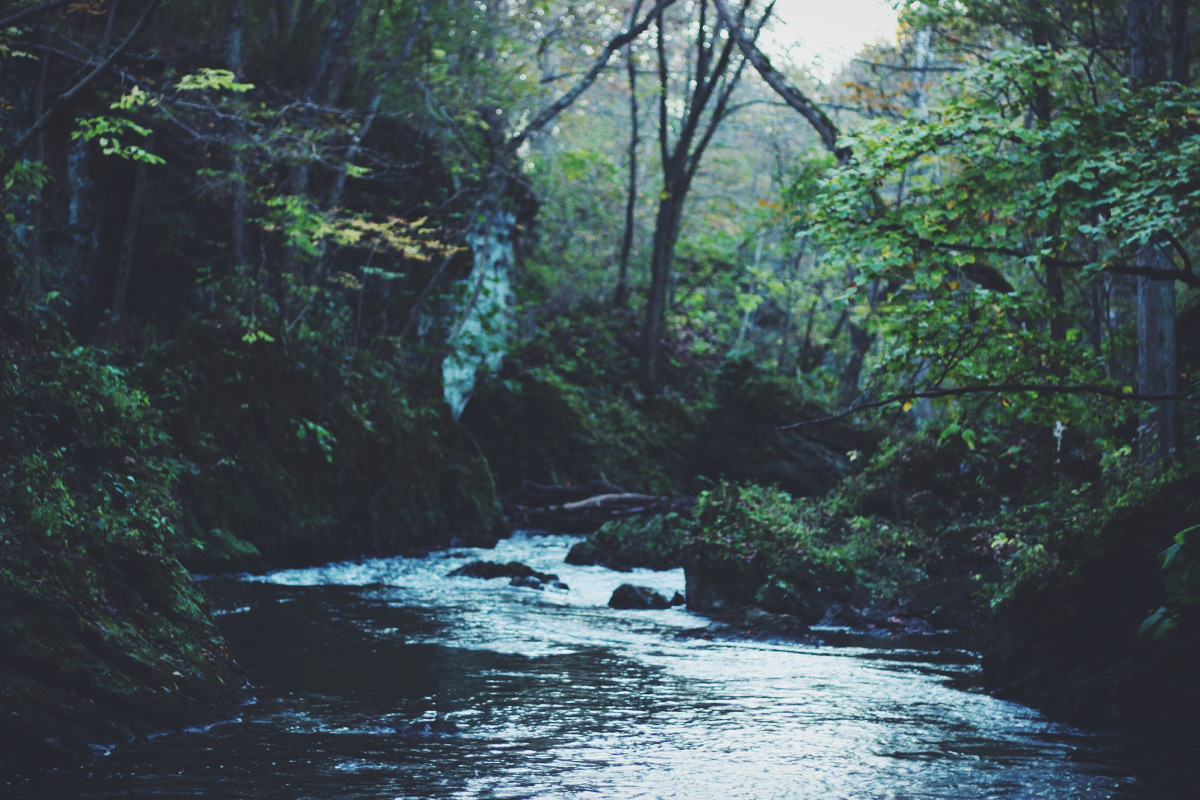
\includegraphics[width=\linewidth]{stream}
\caption{Legend (350 words max). Example legend text.}
\label{fig:stream}
\end{figure}

\begin{table}[ht]
\centering
\begin{tabular}{|l|l|l|}
\hline
Condition & n & p \\
\hline
A & 5 & 0.1 \\
\hline
B & 10 & 0.01 \\
\hline
\end{tabular}
\caption{\label{tab:example}Legend (350 words max). Example legend text.}
\end{table}
\fi

\end{document}
